%%%%%%%%%%%%%%%%%%%%%%%%%%%%%%%%%%%%%%%%%%%%%%%%%%%%%%%%%%%%%%%%%
% !TEX root = interimreport.tex
\clearpage
\chapter{THE LLVM COMPILER}\label{ch:Ch3}
%%%%%%%%%%%%%%%%%%%%%%%%%%%%%%%%%%%%%%%%%%%%%%%%%%%%%%%%%%%%%%%%%
%\vspace*{-12pt} % If no text above section, use this vspacing to lift the whole part to the proper starting point - SBÖ

LLVM is a collection of modular and flexible compiler and toolchain software that can be used to build a wide variety of compilers and other tools. LLVM compilers are organized into a set of libraries that implement the parts of a compiler. There are different front-end libraries a for every language and different back-end libraries for every architecture. There is only one common intermediate representation optimizer that connects specific front-end and back-end.

\begin{figure}
    \centering
    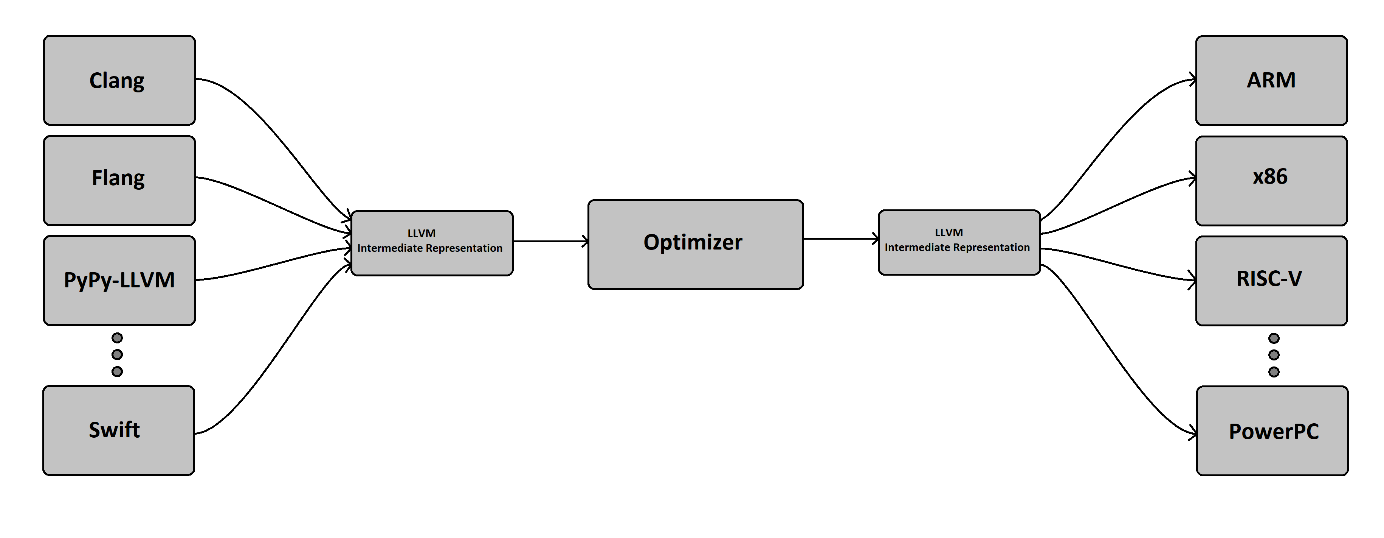
\includegraphics{the_llvm_compiler/llvm_diagram.png}
    \caption{Front-end and Back-end libraries connected by LLVM}
    \label{fig:llvm_diagram}
\end{figure}

LLVM IR is the common representation of languages. Various LLVM front-ends translate related languages into IR. Related back-end compiles IR into assembly according to the target hardware. This structure helps to increase flexibility between front-ends and back-ends. With this structure, we are able to have compilers for every combination of M source codes and N targets with M front-end and N back-end instead of M*N compilers. In our case, we do not have to struggle with the frontend also our backend will be working for every source code of LLVM because of this benefit. The front-end we use in the developing process will be clang which is the LLVM C/C++ front-end\cite{clang}.

\section{Parts of the Clang Frontend}

\subsection{Clang Lex Library}
Clang Lex Library is a typical lexer implemented as finite state machines that read source code one character at a time and transition between different states based on the characters read. The Clang lexer, which is a front-end compiler for the C, C++, and Objective-C programming languages, uses this approach to filter out comments and white space, recognize and tokenize language elements such as keywords, identifiers, and operators, and handle escape sequences and string literals. The implementation files of the Clang lexer can be found in the llvm-project/clang/lib/lex directory within the LLVM infrastructure.
	

\subsection{Clang Parse Library}

Clang Parse Library is the parser that takes the tokens produced by the lexer and constructs an abstract syntax tree (AST) to represent the structure and meaning of the source code. The Clang parser checks the source code for proper syntax and resolves symbols and identifiers. It also performs type-checking to ensure the source code follows the rules of the programming language. It creates the AST, a tree-like structure, that represents the source code in a way that is easily processed by the compiler. The implementation files of the Clang lexer can be found in the llvm-project/clang/lib/parse directory within the LLVM infrastructure.

\subsection{Clang Sema Library}

Clang Sema Library is a semantic analyzer that involves examining the meaning and context of the source code in a program. In Clang, semantic analysis is a phase in the compilation process that analyzes the abstract syntax tree (AST) generated by the parser to verify that the source code conforms to the rules of the programming language and is properly constructed. Semantic analysis performs various checks and transformations on the AST to ensure the source code is correct. The implementation files of the Clang semantic analyzer can be found in the llvm-project/clang/lib/sema directory within the LLVM infrastructure.

\subsection{Clang CodeGen Library}

Clang CodeGen is the code generation library that takes the abstract syntax tree which is generated by the parser and corrected by the semantic analyzer as input. It generates the intermediate representation code and produces .ll file which will be used in the backend. The implementation files of the Clang lexer can be found in the llvm-project/clang/lib/CodeGen directory within the LLVM infrastructure. 

\section{LLVM IR Optimizer}
LLVM Optimizer is a common optimization tool used for every possible source-target combination of a compiler. It takes the output file of CodeGen as input and runs the specified optimizations. The output of the optimizer becomes the input for the RISC-V back-end in our case. LLVM optimizer can be performed with opt [options] [filename] command\cite{optimizer}.

\section{Stages of the LLVM RISC-V Back-end}
LLVM RISC-V Backend is responsible for compiling optimized IR down to RISC-V assembly or object code. LLVM Backend consists of libraries for the code generation steps\cite{llvmbackend}.

\subsection{Instruction Selection}
SelectionDAG is the instruction selector of LLVM backends which is responsible for selecting the appropriate RISC-V instructions for a given intermediate representation instruction. It takes the target-independent LLVM code as input and generates the target-dependent DAG of instructions. SelectionDAG is the most important part of the compiler for us since we will be dealing with adding new instructions to the RISC-V Backend. 

\subsection{Scheduling and Formation}
Scheduling is the phase of assigning an order to the DAG form of RISC-V instructions. The formation phase is responsible for converting the DAG into a list of machine instructions.  

\subsection{SSA-based Machine Code Optimizations}
LLVM uses static single assignment (SSA) based optimizations before register allocation. SSA optimizations ensure that each variable is assigned and defined only once before it is used. 


\subsection{Register Allocation}
The register allocator of RISC-V back-end is responsible for assigning physical registers to virtual registers in the IR. Each target has specific register count and order. Register allocator maps the registers by taking the RISC-V architecture registers into account. It uses the relevant TargetRegisterInfo, and MachineOperand classes. Register allocation will play a key role in our project while we manipulating the implementation of the selected instructions.

\subsection{Prolog/Epilog Code Insertion}
Prolog and epilog code insertion is another optimization phase which is responsible for frame-pointer elimination and stack packing.


\subsection{Code Emission}
Code emission stage is responsible for lowering the code generator abstractions down to the MC layer abstractions. It takes the assembly as input and creates the final RISC-V machine codes. 

\subsection{Linking}
LLD is the LLVM linker library that is responsible for combining multiple object files into a single executable file. LLD is invoked after the code emission and generates a file by resolving symbol references, adjusting addresses, and performing other tasks as necessary.
